\documentclass[12pt]{article}

% ── Packages ──────────────────────────────────────────────────
\usepackage[a4paper, margin=1in]{geometry}
\usepackage{graphicx}
\usepackage{hyperref}
\usepackage{amsmath}
\usepackage{float}
\usepackage{xcolor}
\usepackage{booktabs}
\usepackage{titlesec}
\usepackage{fancyhdr}
\usepackage{enumitem}
\usepackage{array}
\usepackage{mdframed}

% ── Hyperlink Styling ─────────────────────────────────────────
\hypersetup{
    colorlinks = true,
    linkcolor  = blue!60!black,
    urlcolor   = blue!70!black,
    citecolor  = black
}

% ── Section Title Styling ─────────────────────────────────────
\titleformat{\section}
  {\large\bfseries\color{blue!50!black}}
  {\thesection.}{0.6em}{}[\titlerule]

\titleformat{\subsection}
  {\normalsize\bfseries\color{black}}
  {\thesubsection}{0.5em}{}

% ── Header / Footer ───────────────────────────────────────────
\pagestyle{fancy}
\fancyhf{}
\rhead{\textcolor{gray}{\small Machine Learning Practice Report}}
\lhead{\textcolor{gray}{\small CSE Department}}
\cfoot{\thepage}
\renewcommand{\headrulewidth}{0.4pt}

% ── Cover Page Info ───────────────────────────────────────────
\begin{document}

% ═══════════════════════════════════════════════════════════════
%  COVER PAGE
% ═══════════════════════════════════════════════════════════════
\begin{titlepage}
    \centering
    \vspace*{1.2cm}

    {\Huge\bfseries\color{blue!50!black}
        Machine Learning Models:\\[0.3em]
        A Hands-On Practice Report
    \par}

    \vspace{0.8cm}
    \rule{0.7\linewidth}{1.2pt}
    \vspace{0.8cm}

    {\large\textit{Covering: Linear Regression, Logistic Regression,\\
    Support Vector Machines, K-Nearest Neighbors,\\
    Decision Trees, and K-Means Clustering}\par}

    \vspace{1.4cm}

    \begin{mdframed}[linecolor=blue!40!black, linewidth=1pt,
                     innerleftmargin=20pt, innerrightmargin=20pt,
                     innertopmargin=12pt, innerbottommargin=12pt]
    \centering
    {\large\textbf{Submitted by:}}\par\vspace{0.3em}
    {\Large\bfseries Shafikul Islam Marwan}\par\vspace{0.3em}
    {\normalsize ID: 220121}\par\vspace{0.3em}
    {\normalsize Department of Computer Science and Engineering}
    \end{mdframed}

    \vspace{1.2cm}

    \begin{tabular}{rl}
        \textbf{Course:}    & Machine Learning Lab \\[4pt]
        \textbf{Submission Date:} & \today \\[4pt]
    \end{tabular}

    \vfill

    
\includegraphics[width=0.18\textwidth]{Just_Logo.jpeg}   % replace with university logo if available
    \par\vspace{0.4em}
    {\small\textcolor{gray}{Jashore University of Science and Technology}}

\end{titlepage}

% ═══════════════════════════════════════════════════════════════
\tableofcontents
\newpage

% ═══════════════════════════════════════════════════════════════
\section{Introduction}

Machine Learning (ML) occupies a central role in modern data science and artificial intelligence, enabling computer systems to learn patterns directly from data and make informed predictions without being explicitly programmed for every scenario. Rather than relying on hand-crafted rules, ML algorithms iteratively tune internal parameters by optimizing a defined objective function over labelled or unlabelled training data.

This practice report provides a concise walkthrough of six foundational ML techniques implemented using Python's \texttt{scikit-learn} library:

\begin{itemize}[leftmargin=2em, itemsep=4pt]
    \item \textbf{Linear Regression}: a parametric model for continuous target estimation.
    \item \textbf{Logistic Regression}: a probabilistic binary classification framework.
    \item \textbf{Support Vector Machine (SVM)}: a maximum-margin classifier using kernel transformations.
    \item \textbf{K-Nearest Neighbors (KNN)}: a lazy, instance-based proximity classifier.
    \item \textbf{Decision Tree}: a recursive, rule-based hierarchical classifier.
    \item \textbf{K-Means Clustering}: a centroid-driven unsupervised partitioning algorithm.
\end{itemize}

The emphasis of this submission is on practical exposure to LaTeX typesetting and scientific report formatting; deeper mathematical derivations and full pipeline evaluations will follow in the final report.

% ═══════════════════════════════════════════════════════════════
\section{Linear Regression}

\subsection{Objective}
The goal of this module is to fit a continuous predictor that maps one or more input features to a numeric output target by finding the optimal linear relationship between them.

\subsection{Dataset: Diabetes (Scikit-Learn Built-in)}
The \textit{Diabetes} dataset provided by \texttt{sklearn.datasets} was selected for this experiment. It consists of 442 patient records with 10 physiological features (age, sex, BMI, blood pressure, and six serum measurements). The response variable represents a quantitative measure of disease progression one year after baseline. The \textbf{BMI feature} was isolated as the single independent variable to enable a clear two-dimensional visualisation of the regression fit.

\subsection{Data Preparation Steps}
\begin{itemize}[leftmargin=2em, itemsep=3pt]
    \item \textbf{Feature Selection:} Extracted the BMI column (index 2) as the sole predictor variable.
    \item \textbf{Train/Test Split:} Partitioned the data into 80\% training and 20\% testing subsets using a fixed \texttt{random\_state = 7} for reproducibility.
    \item \textbf{No scaling required:} Features in this dataset are already pre-standardised by \texttt{scikit-learn}.
\end{itemize}

\subsection{Mathematical Basis}
The OLS regression model estimates the output $\hat{y}$ using:
\[
\hat{y} = w_1 x_{\text{BMI}} + b
\]
where $w_1$ is the slope coefficient and $b$ is the bias intercept. The training objective is to minimise the \emph{Mean Squared Error} (MSE) loss:
\[
\mathcal{L}_{\text{MSE}} = \frac{1}{n}\sum_{i=1}^{n}(y_i - \hat{y}_i)^2
\]

\subsection{Results}
The fitted regression line is overlaid on the scatter of actual test-set values in Figure~\ref{fig:Linear.png}. The positive slope confirms that higher BMI correlates with greater disease progression.

\begin{figure}[H]
    \centering
    \includegraphics[width=0.82\textwidth]{linear.png}
    \caption{Linear Regression — OLS Best-Fit Line on the Diabetes Dataset (BMI vs.\ Disease Progression Score). Blue dots are actual test-set observations; the red line is the model prediction.}
    \label{fig:linear}
\end{figure}

% ═══════════════════════════════════════════════════════════════
\section{Logistic Regression}

\subsection{Objective}
Logistic Regression extends the linear model to classification tasks by passing the linear combination through a sigmoid function, producing class probabilities bounded in $[0, 1]$.

\subsection{Dataset — Breast Cancer Wisconsin}
The \textit{Breast Cancer Wisconsin} dataset (569 samples, 30 numeric features) was used. Each sample describes characteristics of a digitised image of a fine needle aspirate (FNA) of a breast mass. The binary target labels tumours as either \textit{malignant} (0) or \textit{benign} (1). This is a standard medical classification benchmark with well-balanced classes and clean feature engineering, making it ideal for evaluating logistic models.

\subsection{Data Preparation Steps}
\begin{itemize}[leftmargin=2em, itemsep=3pt]
    \item \textbf{Standardisation:} Applied \texttt{StandardScaler} to bring all 30 features to zero mean and unit variance.
    \item \textbf{Train/Test Split:} Used an 80/20 split with \texttt{random\_state = 42}.
    \item \textbf{Solver:} \texttt{lbfgs} with \texttt{max\_iter = 1000} to ensure convergence.
\end{itemize}

\subsection{Mathematical Basis}
The sigmoid activation maps the linear combination $z = \mathbf{w}^T\mathbf{x} + b$ to a probability:
\[
P(y = 1 \mid \mathbf{x}) = \sigma(z) = \frac{1}{1 + e^{-z}}
\]
Parameters are optimised by minimising the binary cross-entropy loss:
\[
\mathcal{L}_{\text{BCE}} = -\frac{1}{n}\sum_{i=1}^{n}\left[y_i \log \hat{p}_i + (1 - y_i)\log(1 - \hat{p}_i)\right]
\]

\subsection{Results}
The ROC curve in Figure~\ref{fig:Logistic.png} demonstrates excellent separation between the two classes, achieving an AUC close to 1.0, indicating near-perfect discriminative ability on this dataset.

\begin{figure}[H]
    \centering
    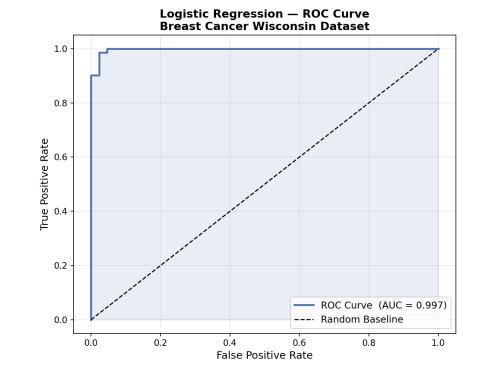
\includegraphics[width=0.72\textwidth]{Logistic.png}
    \caption{ROC Curve for Logistic Regression on the Breast Cancer Wisconsin Dataset. The shaded blue region represents the area under the curve (AUC); higher AUC indicates stronger classifier performance.}
    \label{fig:logistic}
\end{figure}

% ═══════════════════════════════════════════════════════════════
\section{Support Vector Machine (SVM)}

\subsection{Objective}
An SVM seeks the decision boundary (hyperplane) that maximises the geometric margin between the nearest training points of each class, known as \emph{support vectors}. Non-linear separability is handled through the kernel trick.

\subsection{Dataset — Wine Recognition}
The \textit{Wine} dataset (178 samples, 13 chemical features, 3 class labels) was selected. For clean 2D visualisation, only the first two wine varieties (class 0 and class 1) were retained, and the 13 features were compressed to two principal components via PCA before training the SVM.

\subsection{Data Preparation Steps}
\begin{itemize}[leftmargin=2em, itemsep=3pt]
    \item \textbf{Binary Filtering:} Retained only samples belonging to class 0 and class 1.
    \item \textbf{Standardisation:} Applied \texttt{StandardScaler} across all 13 features.
    \item \textbf{Dimensionality Reduction:} Projected onto 2 principal components (PCA) to enable boundary visualisation.
    \item \textbf{Kernel:} Radial Basis Function (RBF) kernel with $C = 1.0$, \texttt{gamma = `scale'}.
\end{itemize}

\subsection{Mathematical Basis}
The SVM optimisation problem seeks to maximise the margin $\tfrac{2}{\|\mathbf{w}\|}$ subject to:
\[
y_i\!\left(\mathbf{w}^T\mathbf{x}_i + b\right) \geq 1 \quad \forall\, i
\]
The RBF kernel implicitly maps inputs to a higher-dimensional space:
\[
K(\mathbf{x}_i, \mathbf{x}_j) = \exp\!\left(-\gamma\,\|\mathbf{x}_i - \mathbf{x}_j\|^2\right)
\]

\subsection{Results}
Figure~\ref{fig:svm} shows the non-linear decision boundary learned by the RBF-SVM in PCA space. Hollow red circles highlight the support vectors that define and anchor the margin boundary.

\begin{figure}[H]
    \centering
    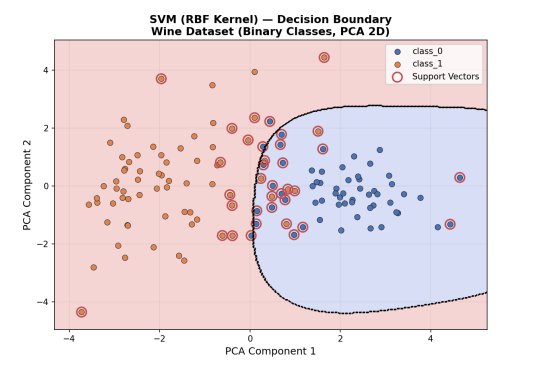
\includegraphics[width=0.80\textwidth]{svm.png}
    \caption{SVM with RBF Kernel — Decision Boundary on the Wine Dataset (Binary, 2D PCA Projection). The dashed boundary separates the two classes; red hollow circles are support vectors.}
    \label{fig:svm}
\end{figure}

% ═══════════════════════════════════════════════════════════════
\section{K-Nearest Neighbors (KNN)}

\subsection{Objective}
KNN is a non-parametric, memory-based classifier that assigns a label to a query point based on the majority vote of its $K$ closest neighbours in the feature space, using a chosen distance metric (typically Euclidean).

\subsection{Dataset — Iris Flower}
The classic \textit{Iris} dataset (150 samples, 4 features, 3 species) was employed. The four features—sepal length, sepal width, petal length, and petal width—were standardised and then projected to 2D via PCA for visualisation. The three target classes (\textit{setosa}, \textit{versicolor}, \textit{virginica}) provide a multi-class challenge that reveals the shape of KNN decision boundaries.

\subsection{Data Preparation Steps}
\begin{itemize}[leftmargin=2em, itemsep=3pt]
    \item \textbf{Standardisation:} \texttt{StandardScaler} applied to ensure equal contribution from all four features to Euclidean distance.
    \item \textbf{PCA Projection:} Reduced to 2 principal components for 2D decision-surface visualisation.
    \item \textbf{Hyperparameter Search:} Tested $K \in \{1, 2, \ldots, 20\}$ and selected the value yielding maximum test accuracy.
\end{itemize}

\subsection{Empirical Observations}
Very small $K$ values (e.g., $K = 1$) lead to jagged, overfitted boundaries sensitive to noise. As $K$ increases, boundaries smooth out. The accuracy-vs-$K$ curve in Figure~\ref{fig:knn} (left) pinpoints the optimal neighbourhood size, while the right panel illustrates the resulting multi-class decision regions.

\begin{figure}[H]
    \centering
    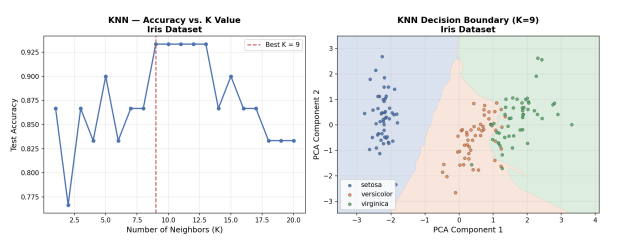
\includegraphics[width=\textwidth]{knn.png}
    \caption{Left: Test accuracy vs.\ $K$ value on the Iris dataset; the dashed red line marks the optimal $K$. Right: KNN decision boundary in the 2D PCA space with colour-coded class regions.}
    \label{fig:knn}
\end{figure}

% ═══════════════════════════════════════════════════════════════
\section{Decision Tree}

\subsection{Objective}
A Decision Tree recursively partitions the feature space by selecting at each node the split that most increases the purity of the resulting subsets. The result is a human-interpretable tree structure that can be directly visualised.

\subsection{Dataset — Breast Cancer Wisconsin}
The same \textit{Breast Cancer Wisconsin} dataset used in Section~3 was re-applied here, now for a non-linear, tree-based approach. With 30 input features and a binary target, it provides a rich partitioning space to benchmark both Gini and Entropy splitting criteria.

\subsection{Splitting Criteria Compared}
\begin{itemize}[leftmargin=2em, itemsep=3pt]
    \item \textbf{Entropy / Information Gain (ID3):}
    \[
    H = -\sum_{c=1}^{C} p_c \log_2 p_c
    \]
    \item \textbf{Gini Impurity (CART):}
    \[
    G = 1 - \sum_{c=1}^{C} p_c^2
    \]
    where $p_c$ is the fraction of training samples belonging to class $c$ within the node.
\end{itemize}

This experiment used \textbf{Entropy} as the splitting criterion with \texttt{max\_depth = 3} to prevent overfitting while keeping the tree interpretable.

\subsection{Results}
Figure~\ref{fig:dtree} shows the tree structure (left) and the resulting confusion matrix on the test set (right). The tree achieves strong accuracy within just three levels of splitting, demonstrating the power of entropy-guided partitioning on well-structured medical data.

\begin{figure}[H]
    \centering
    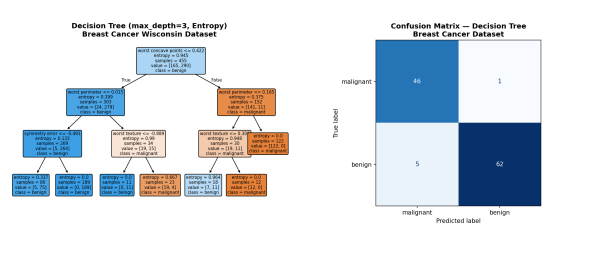
\includegraphics[width=\textwidth]{dtree.png}
    \caption{Left: Visualised Decision Tree (max\_depth = 3, Entropy criterion) trained on the Breast Cancer dataset. Right: Confusion Matrix on the held-out test set; darker blue indicates more correct predictions.}
    \label{fig:dtree}
\end{figure}

% ═══════════════════════════════════════════════════════════════
\section{K-Means Clustering}

\subsection{Objective}
K-Means is an unsupervised algorithm that partitions $n$ observations into $K$ non-overlapping clusters by iteratively assigning each point to its nearest centroid and updating centroid positions until convergence.

\subsection{Dataset — Synthetic Gaussian Blobs}
A synthetic dataset of 400 points arranged in four Gaussian clusters was generated using \texttt{sklearn.datasets.make\_blobs} with \texttt{cluster\_std = 1.0} and \texttt{random\_state = 21}. A controlled synthetic dataset was chosen here because it allows precise verification of cluster recovery — we know the ground-truth number of clusters and can directly assess whether K-Means identifies them correctly.

\subsection{Data Preparation Steps}
\begin{itemize}[leftmargin=2em, itemsep=3pt]
    \item \textbf{Standardisation:} \texttt{StandardScaler} applied to equalise feature scales before distance computation.
    \item \textbf{Elbow Method:} Computed Within-Cluster Sum of Squares (WCSS) for $K \in [1, 10]$ to identify the elbow.
    \item \textbf{Initialisation:} Used \texttt{k-means++} to spread initial centroids, avoiding poor local minima.
\end{itemize}

\subsection{Mathematical Basis}
K-Means minimises the WCSS objective:
\[
J = \sum_{k=1}^{K}\;\sum_{\mathbf{x}_i \in S_k} \|\mathbf{x}_i - \boldsymbol{\mu}_k\|^2
\]
where $S_k$ is the set of points assigned to cluster $k$ and $\boldsymbol{\mu}_k$ is the mean (centroid) of that cluster.

\subsection{Results}
The elbow in Figure~\ref{fig:kmeans} (left) is clearly visible at $K = 4$, matching the true number of blobs. The right panel confirms that the algorithm correctly recovers all four clusters, with centroids (black crosses) positioned near the true generating centres.

\begin{figure}[H]
    \centering
    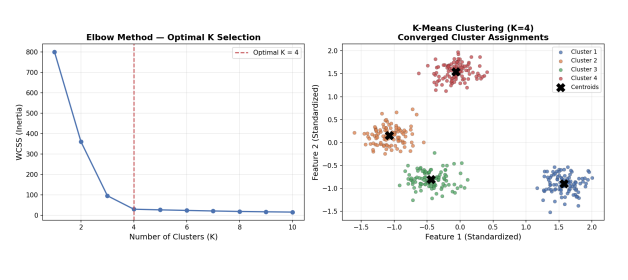
\includegraphics[width=\textwidth]{kmeans.png}
    \caption{Left: Elbow Method plot — WCSS drops sharply up to $K = 4$ and then flattens. Right: Final cluster assignments with four colour-coded groups and black-cross centroids after convergence.}
    \label{fig:kmeans}
\end{figure}

% ═══════════════════════════════════════════════════════════════
\section{Conclusion}

This practice report implemented and visualised six core machine learning algorithms across a variety of dataset types and problem settings. Several practical observations emerged:

\begin{itemize}[leftmargin=2em, itemsep=4pt]
    \item \textbf{Preprocessing is critical:} Distance-sensitive models (KNN, SVM, K-Means) require feature standardisation to function correctly; tree-based methods are scale-invariant but still benefit from clean data.
    \item \textbf{Model interpretability varies:} Decision Trees offer direct visual inspection of learned rules, while SVMs and KNN provide less transparent decision logic.
    \item \textbf{Hyperparameter sensitivity:} KNN accuracy fluctuates noticeably with $K$; K-Means clustering quality depends heavily on the choice of $K$ and the centroid initialisation strategy.
    \item \textbf{Evaluation tools matter:} A single accuracy number is insufficient — ROC-AUC, confusion matrices, and WCSS elbow plots each reveal different aspects of model performance.
\end{itemize}

These foundational experiments establish the groundwork for the final comprehensive report, which will include complete mathematical derivations, full dataset analysis, hyperparameter tuning tables, and detailed evaluation across multiple metrics.

% ═══════════════════════════════════════════════════════════════
\section{References and Resources}

\begin{enumerate}[leftmargin=2em, itemsep=4pt]
    \item Scikit-Learn Documentation and API Reference — \url{https://scikit-learn.org/stable/}
    \item Pedregosa et al., \textit{Scikit-learn: Machine Learning in Python}, JMLR 12, 2011.
    \item UCI Machine Learning Repository — \url{https://archive.ics.uci.edu/ml/index.php}
    \item Kaggle Datasets and Notebooks — \url{https://www.kaggle.com}
    \item Source Code Repository — \url{https://github.com/YourUsername/ml-practice-lab}
\end{enumerate}

\end{document}
